\documentclass[conference]{IEEEtran}
\IEEEoverridecommandlockouts
\usepackage{amsmath,amssymb,amsfonts}
\usepackage{algorithmic}
\usepackage{graphicx}
\usepackage{textcomp}
\usepackage{xcolor}
\usepackage{placeins}
\def\BibTeX{{\rm B\kern-.05em{\sc i\kern-.025em b}\kern-.08em
    T\kern-.1667em\lower.7ex\hbox{E}\kern-.125emX}}
\begin{document}

\title{Robot Navigation in a Simulated Escape Room}

\author{
\IEEEauthorblockN{Student 1}
\IEEEauthorblockA{\textit{Faculty of Informatics}\\
\textit{Università della Svizzera italiana}\\
Lugano, Switzerland}
\and
\IEEEauthorblockN{Student 2}
\IEEEauthorblockA{\textit{Faculty of Informatics}\\
\textit{Università della Svizzera italiana}\\
Lugano, Switzerland}
\and
\IEEEauthorblockN{Student 3}
\IEEEauthorblockA{\textit{Faculty of Informatics}\\
\textit{Università della Svizzera italiana}\\
Lugano, Switzerland}
}

\maketitle

\begin{abstract}
This paper describes an autonomous robot system built for a
simulated escape-room task.
A DJI RoboMaster~EP robot, running in CoppeliaSim, must explore
an unknown room, find a coloured key cylinder, pick it up, and
place it on a pressure plate.
The robot uses only wheel-encoder odometry, a 2D lidar scan,
and a monocular camera.
We built three components on top of ROS~2, Nav2, and slam\_toolbox:
a lidar sensor script injected into the simulator, a colour-based
landmark detector using monocular depth estimation, and a nine-state
mission controller that combines Nav2 path planning with
visual servoing for the pickup.
The robot completes the full task from start to finish.
\end{abstract}

\begin{IEEEkeywords}
autonomous mobile robotics, ROS~2, Nav2, slam\_toolbox,
visual servoing, frontier exploration, monocular depth
\end{IEEEkeywords}

% =====================================================================
\section{Introduction}

This project is an escape-room task in simulation.
A DJI RoboMaster~EP robot is placed in a room with obstacles and
must find a magenta cylinder (the key), pick it up, and drop it on
a green pressure plate to finish.
The room layout and object positions are not known in advance.

\begin{figure}[htbp]
\centerline{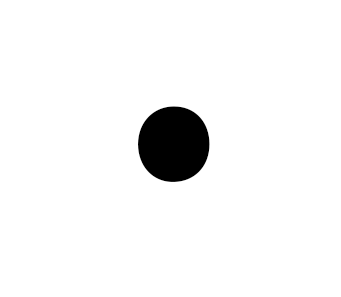
\includegraphics[width=\columnwidth]{fig_scenarios.png}}
\caption{The three scenario variants (easy, medium, hard) shown
from above in CoppeliaSim. Obstacle count and placement increase
across scenarios; the robot spawn, key, and plate positions also
change.}
\label{fig:scenarios}
\end{figure}

The simulation runs in CoppeliaSim with the
\texttt{robomaster\_sim} plugin and \texttt{robomaster\_ros} driver.
We built three custom components on top of
\texttt{slam\_toolbox} and Nav2:
a lidar sensor, a colour detector, and a mission controller.

The rest of the paper is structured as follows.
Section~\ref{sec:arch} explains the overall system.
Sections~\ref{sec:perception}--\ref{sec:mission} describe each component.
Section~\ref{sec:challenges} covers the problems we ran into and how
we fixed them.
Section~\ref{sec:conclusion} concludes.

% =====================================================================
\section{System Architecture}
\label{sec:arch}

\subsection{Simulator--ROS bridge}

CoppeliaSim provides a remote API over ZMQ.
We use it in three places: (1) a scene-building script that constructs
the room from a JSON file at startup; (2) the colour detector reads the
camera field-of-view angle once at startup for the depth calculation;
(3) the mission controller opens and closes the gripper and hides or
shows the cube to the lidar as needed.

\subsection{Node graph and data flow}

\begin{figure}[htbp]
\centerline{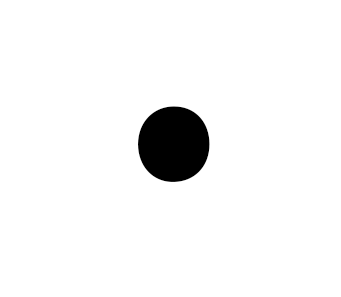
\includegraphics[width=\columnwidth]{fig_architecture.png}}
\caption{Node graph. White boxes: our components. Grey: third-party packages.
Arrows show the main ROS~2 topics and actions between nodes.}
\label{fig:arch}
\end{figure}

Fig.~\ref{fig:arch} shows the data flow between all nodes.

\subsection{Scenario configuration}

The room, obstacles, and task objects are all defined in a JSON file
that is passed to the scene builder at startup.
The file contains: room size and wall thickness; door openings;
a list of obstacles (type, position, size, colour); the key cylinder;
and the pressure plate.
The scene builder connects to CoppeliaSim, removes any previous
objects, and builds the room from scratch.
This means changing the scenario only requires swapping the JSON file,
no code changes are needed.
Two scenarios are included: \texttt{easy.json} (5$\times$4~m room,
three obstacles) and \texttt{medium.json} (same room, four obstacles
with a wall-length divider, offset door, and different robot start).
The colours in the JSON must match the HSV thresholds in the
colour detector.

\subsection{Coordinate frames}

The TF tree is:
\texttt{map\,$\to$\,odom\,$\to$\,base\_link\,$\to$\,laser\_link}.
\texttt{slam\_toolbox} provides \texttt{map\,$\to$\,odom};
\texttt{robomaster\_ros} provides \texttt{odom\,$\to$\,base\_link};
a static publisher provides \texttt{base\_link\,$\to$\,laser\_link}
at $z = 0.12$~m.
The camera frame \texttt{camera\_optical\_link} is also published
by \texttt{robomaster\_ros} and is used by the colour detector to
convert pixel detections to 3D positions.

% =====================================================================
\section{Perception}
\label{sec:perception}

\subsection{Lidar sensor}

CoppeliaSim does not publish laser scans for ROS~2 by default.
We wrote a Lua script that is injected into the simulator at startup
and attached to the robot.
Each cycle (10~Hz) the script rotates a ray sensor to each of
$N = 360$ angles $\theta_i = -\pi + i\,(2\pi/N)$, reads the hit
distance, and publishes the result as a laser scan.
The robot body is made invisible to the ray sensor so that rays
pass through the chassis and only hit walls and obstacles.

\subsection{Colour landmark detection}

To find the three landmarks (cube, plate, door), the colour detector
processes each camera frame in HSV colour space.
For each target it applies a colour mask, finds connected blobs, and
keeps the largest one that exceeds a minimum size.
The colour ranges used are: cube (magenta, $H \in [140,170]$),
plate (green, $H \in [40,80]$), door (blue, $H \in [100,130]$)
(OpenCV convention, $H \in [0,179]$).
Magenta was chosen for the cube because it does not appear in the
floor or wall textures of the simulation.

\begin{figure}[htbp]
\centerline{
\includegraphics[width=\columnwidth]{fig_camera_blob.png}}
\caption{Camera view with HSV blob detection. Coloured overlays show
the detected regions for the cube (magenta), pressure plate (green),
and door (blue). The centroid of each blob is used to estimate
the object's position.}
\label{fig:blob}
\end{figure}

\subsubsection{Depth from known height (cube and door)}

The cube and door are upright objects with known real heights
(0.20~m and 0.50~m).
Using the pinhole camera model, if an object of real height $H$
appears as $h_{\mathrm{px}}$ pixels tall in the image, its depth is:

\begin{equation}
  z = \frac{f \cdot H}{h_{\mathrm{px}}},
  \label{eq:mono}
\end{equation}

where $f$ is the focal length in pixels, computed from the camera
field-of-view angle $\alpha$:
$f = (w/2) / \tan(\alpha/2)$.
The centroid pixel $(c_x, c_y)$ is then converted to a 3D point in
the camera frame:

\begin{equation}
  \mathbf{p}_{\mathrm{cam}} =
  \Bigl(\tfrac{c_x - w/2}{f}\,z,\;\tfrac{c_y - h/2}{f}\,z,\;z\Bigr),
\end{equation}

and transformed to the map frame using the TF tree.
Frames where the blob touches the image edge are skipped because
the pixel height would be cut off and the depth would be wrong.

\subsubsection{Floor-ray intersection (pressure plate)}

The plate is flat on the floor, so measuring its pixel height does
not give a useful depth.
Instead, we shoot a ray through the centroid pixel, transform both
the ray origin and direction to the map frame, and find where the ray
crosses the floor plane ($z = 0$):

\begin{equation}
  s = \frac{-o_z}{p_z - o_z}, \quad
  (x,y) = (o_x + s\,(p_x - o_x),\; o_y + s\,(p_y - o_y)),
\end{equation}

where $\mathbf{o}$ is the camera origin and $\mathbf{p}$ is a point
one unit along the ray, both in the map frame.
This works regardless of the plate's size.

\subsubsection{Live cube position for the pickup}

The cube position in the robot frame (\texttt{base\_link}) is also
published every frame on a separate topic.
The pickup controller uses this to always have a fresh direction
towards the cube.

% =====================================================================
\section{Navigation and Mapping}
\label{sec:nav}

\subsection{SLAM}

\texttt{slam\_toolbox} runs in online mode and
builds a 2D occupancy map at 5~cm per cell from the lidar scan and
odometry.
We disabled loop closure because in a small 5$\times$4~m room it
caused sudden jumps in the map transform when the robot passed through
the same area twice.
Those jumps caused Nav2 to abort its current goal.
Without loop closure, the map is accurate enough for the task.

\begin{figure}[htbp]
\centerline{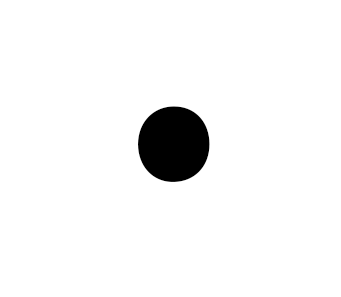
\includegraphics[width=\columnwidth]{fig_map.png}}
\caption{Occupancy grid map built by slam\_toolbox during exploration.
White cells are free space, black cells are obstacles, and grey is
unexplored. The planned path from Nav2 is shown in green.}
\label{fig:map}
\end{figure}

\subsection{Nav2}

Nav2 handles all long-range path planning and following.
We use the NavFn planner (Dijkstra) with a 0.5~m goal tolerance and
the Regulated Pure Pursuit controller at 0.15~m/s.
The local costmap is a 2$\times$2~m rolling window with 0.35~m
inflation around obstacles.
The global costmap covers the full map.

\subsection{Frontier exploration}

To explore the room the robot uses frontier-based
exploration.
A frontier cell is a free cell (map value 0) that has at least one
unknown neighbour (map value $-1$).
Adjacent frontier cells are grouped into clusters using BFS;
clusters with fewer than 20 cells are ignored.
The robot always drives to the closest cluster centre.
Exploration stops once all three landmarks have been seen.

% =====================================================================
\section{Mission Execution}
\label{sec:mission}

\subsection{State machine}

\begin{figure}[htbp]
\centerline{
\includegraphics[width=\columnwidth]{fig_fsm.png}}
\caption{Mission state machine. Shaded states use Nav2 for driving;
white states use direct velocity commands.}
\label{fig:fsm}
\end{figure}

The mission controller (Fig.~\ref{fig:fsm}) runs as a state machine
at 4~Hz.
It waits at startup until Nav2, the map, and the robot position are
all available, then runs through nine states:
\textbf{EXPLORE} $\to$ \textbf{GO\_TO\_KEY} $\to$
\textbf{PICKUP\_OPEN} $\to$ \textbf{PICKUP\_ALIGN} $\to$
\textbf{PICKUP\_CLOSE} $\to$ \textbf{GO\_TO\_PLATE} $\to$
\textbf{DROP\_ALIGN} $\to$ \textbf{DROP\_OPEN} $\to$
\textbf{DROP\_BACKUP} $\to$ \textbf{DONE}.

\subsection{Navigation states}

\textbf{GO\_TO\_KEY} sends a Nav2 goal to a point 0.9~m in front of
the cube, facing it.
\textbf{GO\_TO\_PLATE} sends a goal to the plate position.
If Nav2 fails (for example, a partial plan near a wall), the goal
is retried automatically.

\begin{figure}[htbp]
\centerline{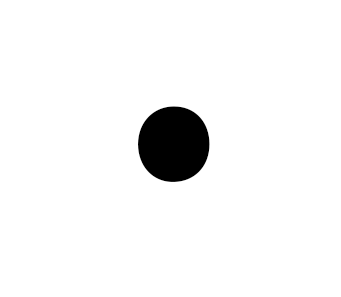
\includegraphics[width=\columnwidth]{fig_stage_explore.png}}
\caption{EXPLORE state: the robot drives toward the nearest frontier
while slam\_toolbox builds the map. The planned path and current
costmap are visible in RViz.}
\label{fig:stage_explore}
\end{figure}

\FloatBarrier
\subsection{Pickup (PICKUP\_ALIGN)}

The pickup works in two steps.
First, the robot uses the live cube position from the camera:
it turns to face the cube and drives forward while keeping it centred
(proportional control on the yaw error).

At about 0.9~m from the cube, the bottom of the 0.20~m cylinder
moves below the camera's field of view.
At that point the pixel height $h_\mathrm{px}$ in~\eqref{eq:mono}
becomes wrong, so the depth estimate is no longer reliable.
The robot therefore switches to an \emph{odometry lunge}: it drives
straight ahead by a fixed distance measured from the odometry, not
from SLAM (the SLAM map transform can jump, while odometry is smooth
over short distances).
The lunge distance is:
$d_\mathrm{lunge} = r - d_\mathrm{engage} - d_\mathrm{margin}$,
where $r = 0.9$~m is the frozen range, $d_\mathrm{engage} = 0.177$~m
is the gripper reach, and $d_\mathrm{margin} = 0.03$~m avoids
tipping the thin cylinder.
The gripper then closes.

\begin{figure}[htbp]
\centerline{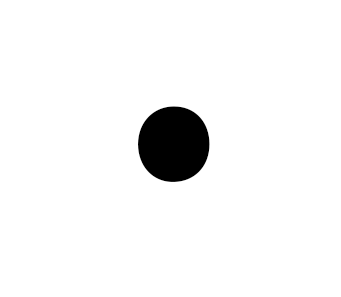
\includegraphics[width=\columnwidth]{fig_stage_pickup.png}}
\caption{PICKUP\_ALIGN state: the robot approaches the magenta
cylinder using visual servoing. The camera view (inset) shows the
cube centred in the frame just before the odometry lunge.}
\label{fig:stage_pickup}
\end{figure}

While the cube is being carried, it is hidden from the lidar so that
Nav2 does not see it as a wall in front of the robot.

\FloatBarrier
\subsection{Drop (DROP\_ALIGN, DROP\_OPEN, DROP\_BACKUP)}

\begin{figure}[htbp]
\centerline{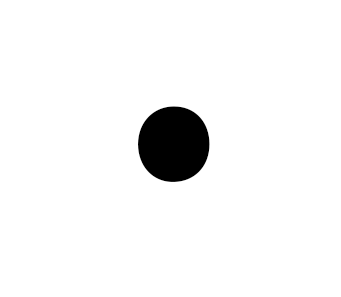
\includegraphics[width=\columnwidth]{fig_stage_drop.png}}
\caption{DROP\_OPEN state: the cube has been placed on the green
pressure plate. The robot is backing away before turning.}
\label{fig:stage_drop}
\end{figure}

Nav2's position tolerance of 0.25~m is too large for a 0.3~m plate.
After arriving near the plate, the robot switches to direct velocity
control for the final alignment: it faces the plate and drives until
the cube's estimated position (gripper reach ahead of the robot)
matches the plate centre, within 0.03~m.
The gripper then opens and the cube becomes visible to the lidar again.
Finally the robot reverses 0.25~m in a straight line before turning,
so that the gripper does not push the cube off the plate.

% =====================================================================
\FloatBarrier
\section{Engineering Challenges}
\label{sec:challenges}

\subsection{Replacing a custom stack with Nav2 and slam\_toolbox}

The first version used a script that read all object positions from
the simulator directly, published them as perfect odometry, and used
a custom Python mapper with an A* planner.
This worked but was unreliable: timing problems in the API calls
corrupted the pose, and the mapper had no scan matching.
We replaced everything with \texttt{slam\_toolbox} and Nav2, using
real wheel-encoder odometry.
This was a lot of work to configure (costmaps, controller tuning,
recovery behaviours) but gave us a much more reliable system.

\subsection{Lidar: Python node to Lua script}

The first lidar was a Python ROS~2 node that asked the simulator for
distances to each obstacle one by one.
This was slow and depended on knowing the object list in advance.
We replaced it with a Lua script running inside the simulator that
rotates a native ray sensor and reads distances directly.
This is much faster and works for any scene.

\subsection{Colour detector: fixing the coordinate transform}

The first version of the colour detector estimated positions in the
robot's local frame using a manual rotation based on the starting
heading.
This broke as soon as the robot turned.
We rewrote it to use the full TF tree, transforming each detection
from the camera frame to the map frame.
This works at any robot pose.

\subsection{Loop closure jumping}

With loop closure enabled, \texttt{slam\_toolbox} sometimes applied a
large correction to the map transform when the robot revisited a
known area.
This moved the robot's estimated position by 0.3--0.5~m instantly,
which made Nav2 abort its current goal.
We disabled loop closure.
The map quality did not noticeably worsen in this small room.

\subsection{Pickup: waypoint to visual servo to odometry lunge}

The first pickup strategy drove to a fixed position offset from the
cube's known location.
The gripper missed often because the position estimate was off by
5--10~cm.
We switched to visual servoing, which keeps the cube centred in the
camera during the approach and does not depend on map accuracy.

We then found a second problem: below 0.9~m, the cylinder base
disappears from the camera's view, making the depth estimate
unreliable.
We added the odometry lunge to handle this last stretch, where
odometry is accurate enough for the short straight-line distance
involved.

\subsection{CoppeliaSim Euler angle bug}

When setting object orientations using Euler angles, CoppeliaSim
silently reorders the angles in some cases (swapping roll and yaw),
so the robot spawned facing the wrong direction.
We fixed this by using the rotation matrix API instead, which has
no ambiguity.

\subsection{Too many files in the mission node}

As we added states, the mission node grew to 13 files.
It became harder to understand and debug than if everything had
been in fewer files.
We reorganised it down to 5 files.
Splitting code into many small files was not worth it for a project
of this size.

% =====================================================================
\section{Conclusion}
\label{sec:conclusion}

We built an autonomous robot system that solves a simulated
escape-room task: it explores an unknown room, finds three
colour-coded objects, picks up the key cylinder with visual
servoing, and drops it on the pressure plate.

The main lesson is that using an existing stack (Nav2 and
slam\_toolbox) is much better than building a custom planner,
even though configuring it took significant effort.
The visual-servo pickup and the odometry lunge were necessary to
make the manipulation reliable, because map-based position estimates
were not accurate enough close to the object.

Future improvements could include better recovery when the cube is
dropped during transport, support for multi-room layouts, or a
depth camera to make the pickup more robust.

\end{document}
